\documentclass[12pt,a4paper]{article}
\usepackage{cmap} % Makes the PDF copiable. See http://tex.stackexchange.com/a/64198/25761
\usepackage[T1]{fontenc}
\usepackage[brazil]{babel}
\usepackage[utf8]{inputenc}
\usepackage{amsmath}
\usepackage{amsfonts}
\usepackage{amssymb}
\usepackage{amsthm}
\usepackage[usenames,svgnames,dvipsnames]{xcolor}
\usepackage{hyperref}
\usepackage{multicol}
\usepackage{graphicx}
\usepackage[top=2cm, bottom=2cm, left=2cm, right=2cm]{geometry}
\usepackage{cancel}

\hypersetup{
    colorlinks = true,
    allcolors = {blue}
}

% TODO: Consider using exsheets
% http://linorg.usp.br/CTAN/macros/latex/contrib/exsheets/exsheets_en.pdf
%
% http://ctan.org/tex-archive/macros/latex/contrib/exercise/
% Options: answerdelayed,lastexercise,noanswer
\usepackage[answerdelayed,lastexercise]{exercise}

\addto\captionsbrazil{%
\def\listexercisename{Lista de exerc\'icios}%
\def\ExerciseName{Exerc\'icio}%
\def\AnswerName{Solu\c{c}\~ao do exerc\'icio}%
\def\ExerciseListName{Ex.}%
\def\AnswerListName{Solu\c{c}\~ao}%
\def\ExePartName{Parte}%
\def\ArticleOf{de\ }%
}

\renewcommand{\ExerciseHeaderTitle}{(\ExerciseTitle)\ }
\renewcommand{\ExerciseListHeader}{%\ExerciseHeaderDifficulty%
\textbf{%\ExerciseListName\
\ExerciseHeaderNB.\ %
%\ --- \
\ExerciseHeaderTitle}%
%\ExerciseHeaderOrigin
\ignorespaces}
\renewcommand{\AnswerListHeader}{\textbf{\ExerciseHeaderNB.\ (\AnswerListName)\ }}

\newcommand*\diff{\mathop{}\!\mathrm{d}}
\newcommand*\sen{\operatorname{sen}}
\newcommand*\R{\mathbb{R}}

\renewcommand{\theenumi}{\alph{enumi}}
\renewcommand\labelenumi{(\theenumi) }

\newcommand*\tipo{Prova II}
\newcommand*\turma{NEXM241-D}
\newcommand*\disciplina{CDI1001}
\newcommand*\eu{Helder G. G. de Lima}
\newcommand*\data{13/05/2024}

\author{\eu}
\title{\tipo - \disciplina}
\date{\data}

\begin{document}
\thispagestyle{empty}
\newgeometry{margin=2cm,bottom=0.5cm}
\begin{center}

\includegraphics[width=9.0cm]{marca} \\
\textbf{\tipo\ (\disciplina / \turma)} \\
Prof. \eu\footnote{
Este é um material de acesso livre distribuído sob os termos da licença \href{https://creativecommons.org/licenses/by-sa/4.0/deed.pt_BR}{Creative Commons BY-SA 4.0}}
\end{center}

\noindent Nome do(a) aluno(a): \underline{\hspace{9,7cm}} Data: \underline{\data}

%\section*{Instruções}
\begin{center}\fbox{
\begin{minipage}{14cm}

{\footnotesize
\begin{itemize}
\renewcommand{\theenumi}{\Roman{enumi}}
\item Identifique-se em todas as folhas.
\item Mantenha o celular e os demais equipamentos eletrônicos desligados durante a prova.
\item Justifique cada resposta com cálculos ou argumentos baseados na teoria estudada.
\item Resolva $5$ das $6$ questões (deixe claro que questão não deverá ser corrigida).
\end{itemize}
}

\end{minipage}
}
\end{center}

%\section*{Questões}
\begin{ExerciseList}
\Exercise[title={2,0}] Calcule, se existir, $\displaystyle \lim_{x \to 4} \frac{e^{x-4}-1}{e^{4-x}-1}$.
\Answer \textbf{Alternativa 1}:
\begin{align*}
      \lim_{x \to 4} \frac{e^{x-4}-1}{e^{4-x}-1}
  & = \lim_{u \to 0} \frac{e^{u}-1}{e^{-u}-1}
    = \lim_{u \to 0} \frac{\frac{e^{u}-1}{u}}{\frac{e^{-u}-1}{u}}
    = \frac{\lim_{u \to 0} \frac{e^{u}-1}{u}}{\lim_{u \to 0} \frac{e^{-u}-1}{u}}
    = \frac{1}{\lim_{t \to 0}  \frac{e^{t}-1}{-t}} \\
  & = \frac{1}{\lim_{t \to 0} -\frac{e^{t}-1}{t}}
    = \frac{1}{-\lim_{t \to 0} \frac{e^{t}-1}{t}}
    = \frac{1}{-1}
    = -1.
\end{align*}

\textbf{Alternativa 2}: Considerando $v = e^{4-x} - 1$, tem-se $v\to 0$ quando $x\to 4$. Além disso, $v + 1 = e^{4-x} = \frac{e^4}{e^x}$, então $e^x = \frac{e^4}{v + 1}$ e $e^{x-4} = \frac{e^x}{e^4} = \frac{1}{v + 1}$. Assim,
\begin{align*}
      \lim_{x \to 4} \frac{e^{x-4}-1}{e^{4-x}-1}
  & = \lim_{v \to 0} \frac{\frac{1}{v+1}-1}{v}
    = \lim_{v \to 0} \frac{\frac{-v}{v+1}}{v}
    = \lim_{v \to 0} \frac{-\cancel{v}}{(v+1)\cancel{v}}
    = \lim_{v \to 0} \frac{-1}{v+1}
    = -1.
\end{align*}

\textbf{Alternativa 3}: Considerando $w = x-4$, tem-se $w\to 0$ quando $x\to 4$. Além disso, $-w = 4-x$, então
\begin{align*}
      \lim_{x \to 4} \frac{e^{x - 4}-1}{e^{4 - x}-1}
  & = \lim_{w \to 0} \frac{e^{w} - 1}{e^{-w} - 1}
    = \lim_{w \to 0} \frac{e^{w} - 1}{e^{-w} - 1}\cdot \frac{e^{w}}{e^{w}}
    = \lim_{w \to 0} \frac{\cancel{(e^{w} - 1)}e^w}{\cancel{1 - e^w}}
    = \lim_{w \to 0} (-1)e^w
    = -1.
\end{align*}

A figura a seguir mostra o gráfico da função $f:\mathbb{R}\setminus\{4\}\to\mathbb{R}$ definida por $f(x) = \frac{e^{x-4}-1}{e^{4-x}-1}$:

\begin{center}
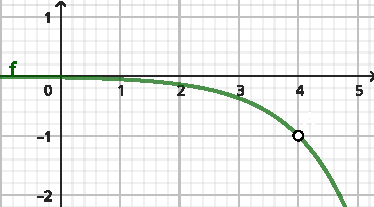
\includegraphics[width=5cm]{img/prova-2-nex-limite.pdf}
\end{center}


\Exercise[title={2,0}] Verifique se a função $g$ é contínua em $x = 0$, sendo
\[
g(x) =
\begin{cases}
  \sqrt{3 + e^x} &, \text{ se } x \geq 0, \\
  \frac{\sen(2x)}{x} &, \text{ se } x < 0.
\end{cases}
\]
\Answer A continuidade de $g$ em $x=0$ equivale a $\lim_{x \to 0} g(x) = g(0)$. No entanto, como $g$ tem fórmulas diferentes para $x \geq 0$ e para $x < 0$, é preciso considerar os limites laterais, que devem ter o mesmo valor.

Para $x > 0$, tem-se:

\[
  \lim_{x \to 0+} \sqrt{3 + e^x} = \sqrt{3 + e^0} = \sqrt{3 + 1} = \sqrt{4} = 2 = g(0)
\]

Para $x < 0$ há duas soluções possíveis:

\textbf{Alternativa 1}:
\[
    \lim_{x \to 0} \frac{\sen(2x)}{x}
  = \lim_{x \to 0} 2\cdot \frac{\sen(2x)}{2x}
  = \lim_{u \to 0} 2\cdot \frac{\sen(u)}{u}
  = 2 \lim_{u \to 0} \cdot \frac{\sen(u)}{u}
  = 2 \cdot 1
  = 2
  = g(0).
\]
\textbf{Alternativa 2}:
\[
    \lim_{x \to 0} \frac{\sen(2x)}{x}
  = \lim_{x \to 0} \frac{2\cos(x)\sen(x)}{x}
  = \lim_{u \to 0} 2\cos(x) \cdot \lim_{u \to 0}\frac{\sen(x)}{x}
  = 2 \cdot 1
  = 2
  = g(0).
\]

A figura a seguir mostra o gráfico da função $g$:

\begin{center}
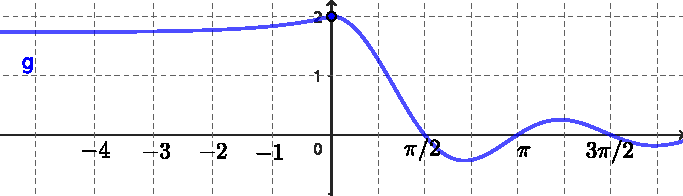
\includegraphics[width=8cm]{img/prova-2-nex-função-por-partes.pdf}
\end{center}


\Exercise[title={2,0}] Seja $f: \left[\frac{1}{5}, +\infty\right) \to \R$ a função dada por $f(x) = \sqrt{5x - 1}$
\begin{enumerate}
\item (1,0 ponto) Calcule $f^\prime(2)$ usando a definição de derivada (isto é, por meio de um limite).\color{black}
\item (1,0 ponto) Utilize as regras de derivação para verificar que a resposta anterior está correta.
\end{enumerate}

\Answer
\begin{enumerate}
\item
\begin{align*}
f^\prime(2)
& = \lim_{h \to 0} \frac{\sqrt{5\cdot (2+h) - 1} - \sqrt{5\cdot 2 - 1}}{h}
  = \lim_{h \to 0} \frac{\sqrt{5h + 9} - 3}{h} \\
& = \lim_{h \to 0} \frac{\sqrt{5h + 9} - 3}{h} \cdot \frac{\sqrt{5h + 9} + 3}{\sqrt{5h + 9} + 3}
  = \lim_{h \to 0} \frac{(5h + 9) - 3^2}{h (\sqrt{5h + 9} + 3)} \\
  &
  = \lim_{h \to 0} \frac{5\cancel{h}}{\cancel{h}\sqrt{5h + 9} + 3}
  = \frac{5}{\sqrt{5\cdot 0 + 9} + 3}
  = \frac{5}{6}.
\end{align*}
\item Como $f(x) = \sqrt{5x - 1}$, tem-se $f^\prime(x) = \frac{1}{2\sqrt{5x - 1}} \cdot (5x - 1)^\prime = \frac{5}{2\sqrt{5x - 1}}$, para todo $x > \frac{1}{5}$. Em particular, em $x = 2$ tem-se $f^\prime(2) = \frac{5}{2 \sqrt{5 \cdot 2 - 1}} = \frac{5}{6}$, que é o mesmo resultado obtido acima.
\end{enumerate}

\Exercise[title={2,0}] Sabendo que a função $h(x) = 4x^3 - \ln(x) + \frac{1}{x^2}$ é derivável em $x_0 = 1$, obtenha a equação da reta tangente ao gráfico de $h$ no ponto $(x_0, h(x_0))$.
\Answer Como
\[
  h^\prime(x)
  = \left(4x^3 - \ln(x) + \frac{1}{x^2}\right)^\prime
  = 4\cdot\left(x^3\right)^\prime - \left(\ln(x)\right)^\prime + \left(\frac{1}{x^2}\right)^\prime
  = 4\cdot 3x^2 - \frac{1}{x} + \frac{-2x}{(x^2)^2}
  = 12x^2 - \frac{1}{x} - \frac{2}{x^3},
\]
para todo $x > 0$, tem-se $h^\prime(1) = 12\cdot 1^2 - \frac{1}{1} - \frac{2}{1^3} = 9$. Além disso,
\[
  h(x_0) = h(1) = 4\cdot 1^3 - \ln(1) + \frac{1}{1^2} = 5,
\]
então, a reta tangente é $y-5 = 9 (x-1)$, ou seja, $y = 9x-4$. A figura a seguir mostra o gráfico da função:
\begin{center}
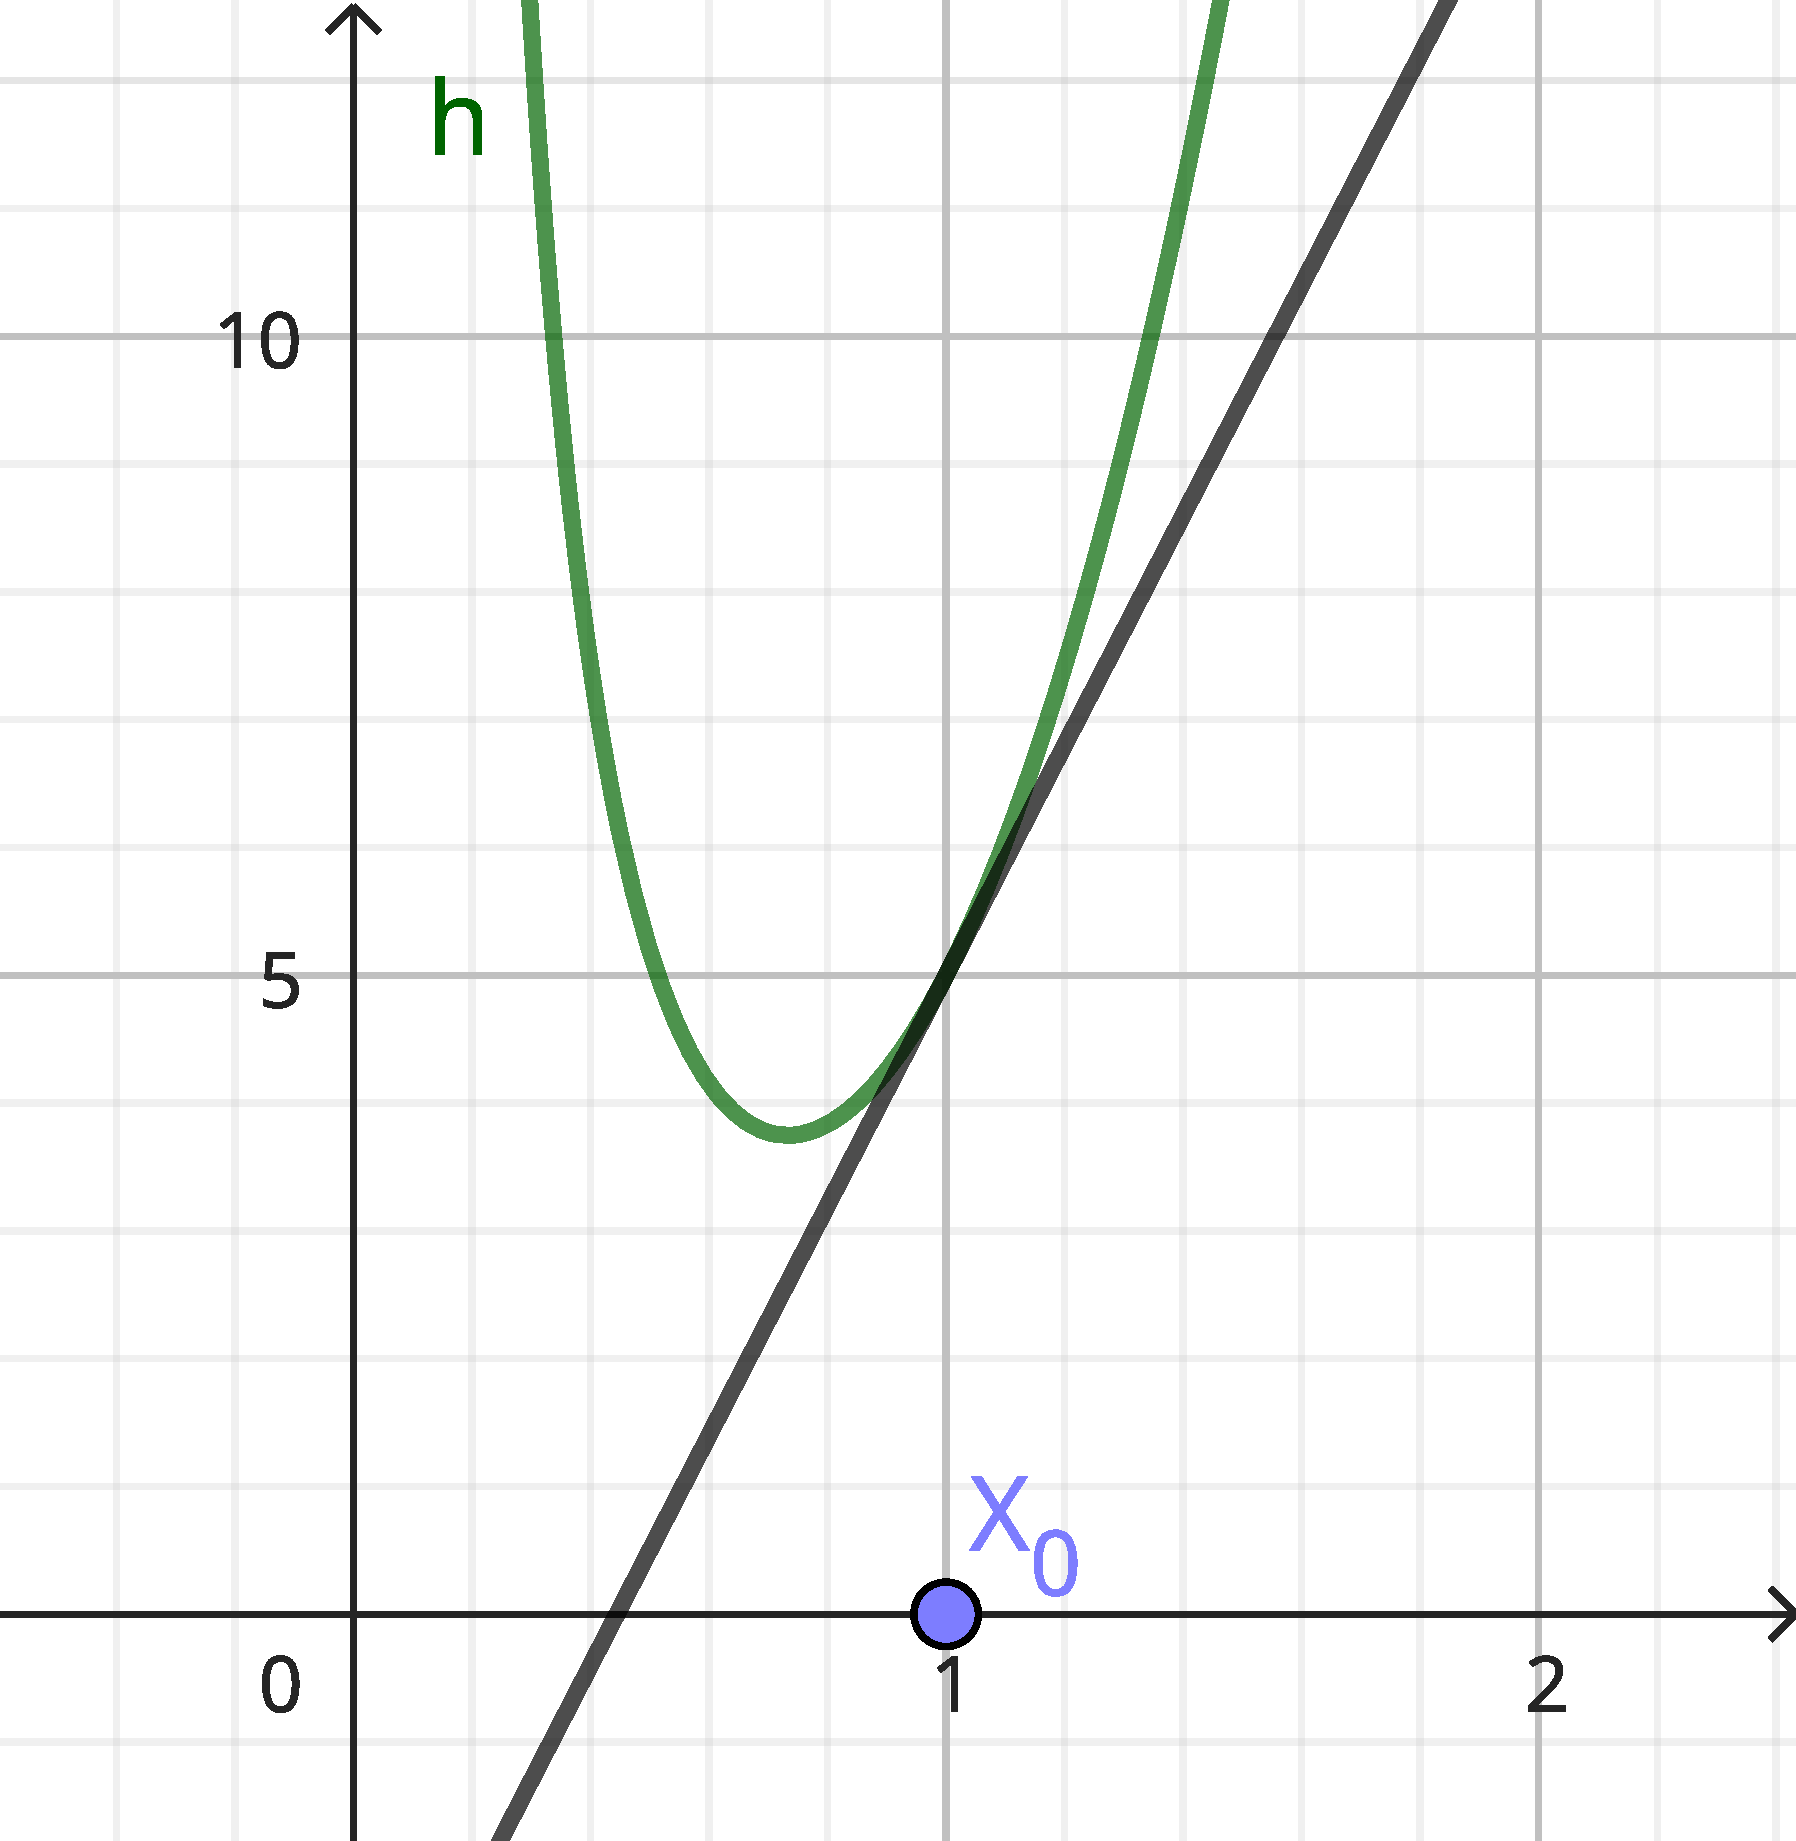
\includegraphics[width=5cm]{img/prova-2-nex-reta-tangente.pdf}
\end{center}


\Exercise[title={2,0}] Seja $y=f(x)$ uma função derivável definida implicitamente pela equação $e^{xy} = 2y$.
\begin{enumerate}
\item (1,5 ponto) Expresse a derivada $y^\prime = \frac{\diff{y}}{\diff{x}}$ em termos de $x$ e $y$.
\item (0,5 ponto) Utilize o resultado anterior para calcular a derivada de $f$ em zero, isto é, $f^\prime(0)$.
\end{enumerate}

\Answer
\begin{enumerate}
\item Considerando que ambos os membros de $e^{xy} = 2y$ são funções deriváveis, e utilizando a regra da cadeia, obtém-se:
\begin{align*}
  \frac{\diff}{\diff{x}} \left(e^{xy}\right) = \frac{\diff{}}{\diff{x}}(2y)
  & \Rightarrow
  e^{xy} \cdot \frac{\diff}{\diff{x}} \left(xy\right) = 2 \cdot \frac{\diff{y}}{\diff{x}}
  \Rightarrow
  e^{xy} \cdot \left(1 \cdot y + x \cdot \frac{\diff{y}}{\diff{x}} \right) = 2 \frac{\diff{y}}{\diff{x}} \\
  & \Rightarrow
  e^{xy} y + e^{xy}x \frac{\diff{y}}{\diff{x}} = 2 \frac{\diff{y}}{\diff{x}}
  \Rightarrow
  e^{xy}x \frac{\diff{y}}{\diff{x}} - 2 \frac{\diff{y}}{\diff{x}} = -e^{xy} y \\
  & \Rightarrow
  \left( e^{xy}x - 2 \right) \frac{\diff{y}}{\diff{x}} = -e^{xy} y
  \Rightarrow
  \frac{\diff{y}}{\diff{x}}
  = \frac{-e^{xy} y}{e^{xy}x - 2}
  = \frac{e^{xy} y}{2- e^{xy}x}.
\end{align*}
\item Em particular, se $x=0$, tem-se
\[
  f^\prime(0)
  = \frac{\diff{y}}{\diff{x}}(0)
  = - \frac{e^{0 \cdot y} y}{2 - e^{0 \cdot y} \cdot 0}
  = \frac{y}{2}.
\]
Substituindo $x=0$ na equação $e^{xy} = 2y$, tem-se $e^{0 \cdot y} = 2y$, ou seja, $y = \frac{1}{2}$. Logo, $f^\prime(0) = \frac{\frac{1}{2}}{2} = \frac{1}{4}$.
\end{enumerate}

A figura a seguir mostra parte do gráfico da curva:
\begin{center}
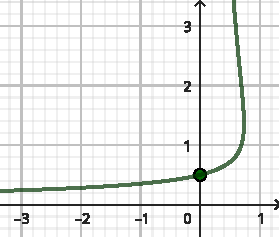
\includegraphics[width=5cm]{img/prova-2-nex-função-implícita.pdf}
\end{center}


\Exercise[title={2,0}] Calcule a derivada da função $y = \arccos(x)$, simplificando sua resposta.
\Answer Como $y = \arccos(x)$ é a função inversa da função cosseno, tem-se:
\[
  y^\prime
  = \frac{1}{\cos^\prime(\arccos(x))}
  = \frac{1}{-\sen(\arccos(x))}
  = \frac{1}{-\sqrt{1 - \cos^2(\arccos(x))}}
  = \frac{-1}{\sqrt{1 - x^2}}.
\]
\end{ExerciseList}

\begin{center}
BOA PROVA!
\end{center}

\newpage
\restoregeometry
\section*{Respostas}
\shipoutAnswer
\end{document}
